\documentclass[12pt]{article}

\usepackage[spanish]{babel}
\usepackage{amsmath}
\usepackage{amssymb}
\usepackage[margin=1in]{geometry}

\usepackage{graphicx}
\graphicspath{{./imagenes/}}

\title{Simulación\\
	\large Práctica de Sistemas Continuos {-} Ejercicio 5}
\author{Pablo Rossi, D'Autilio Joel}
\date{}

\newcommand{\fent}{F_\text{entrada}}
\newcommand{\fsal}{F_\text{salida}}
\newcommand{\fosc}{F_\text{oscilante}}

\begin{document}

\maketitle

\section*{Problema}

En la Figura \ref{ima:tanque} se muestra un sistema de tanque con un canal de salida. Nuestro objetivo es predecir la altura del líquido en el tanque en función del tiempo, es decir, el comportamiento de una función denominada en adelante como $h(t)$.

\begin{figure}
	\centering
	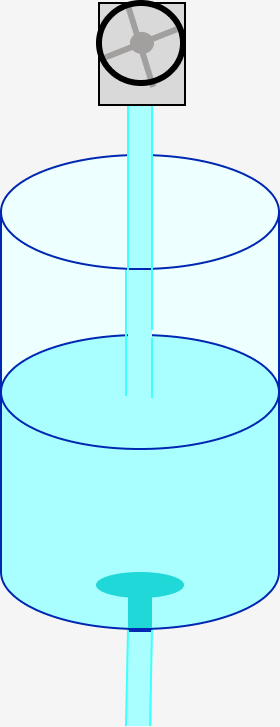
\includegraphics[width=0.2\textwidth]{tanque}
	\caption{Sistema de tanque con canal de salida}
	\label{ima:tanque}
\end{figure}

El área de la base del tanque ($A$) es constante, por lo que solo afectarán al cálculo de la altura dos variables clave: el caudal de entrada al tanque (representado por la función $\fent(t)$) y el caudal de salida de líquido (representado por la función $\fsal(t)$). A continuación se presenta la función $h(t)$:

\[ h(t) = \frac{1}{A} \int_{t_0}^t (\fent(t) - \fsal(t) dt) + h_\text{inicial} \]

Entonces, la ecuación diferencial utilizada para predecir el comportamiento de $h(t)$ es la siguiente:

\[ \frac{dh}{dt} = \frac{1}{A} (\fent(t) - \fsal(t)) \]

La función $\fsal$ depende de la cantidad de líquido en el tanque en el tiempo $t$. A medida que aumenta el volumen, el caudal de salida también aumenta. Es por esto que,  $\fsal(t)$ está directamente relacionada con $h(t)$:

\[ \fsal(t) = K \sqrt{g h(t)} \]

donde $g$ es la gravedad y $K$ es un factor multiplicativo.

Para llevar a cabo este experimento, se consideraron los siguientes valores iniciales:

\begin{align*}
	A & = 2 & K & = 1 & g & = 9.8 & h_\text{inicial} & = 0
\end{align*}

Con estos valores, el objetivo principal es predecir la variación de la altura del líquido en el tiempo para diferentes funciones de entrada $(\fent)$. Para cada comportamiento de entrada adoptado, se graficarán las funciones correspondientes a: $h(t)$, $\fsal(t)$ y $\fent(t)$.


\section*{Resultados}


\subsection*{Función de entrada constante}

En las figuras \ref{gr:c20k0.5}, \ref{gr:c20k1} y \ref{gr:c20k2} se muestran los resultados obtenidos para una función de entrada constante. En todos los casos, el caudal de entrada es de 20 unidades. Esto causa que el agua descienda desde su altura inicial (500) hasta un punto de estabilización. En ese punto, el sistema se estabiliza y la altura se mantiene constante.

\begin{figure}[h]
	\begin{minipage}{0.32\textwidth}
		\centering
		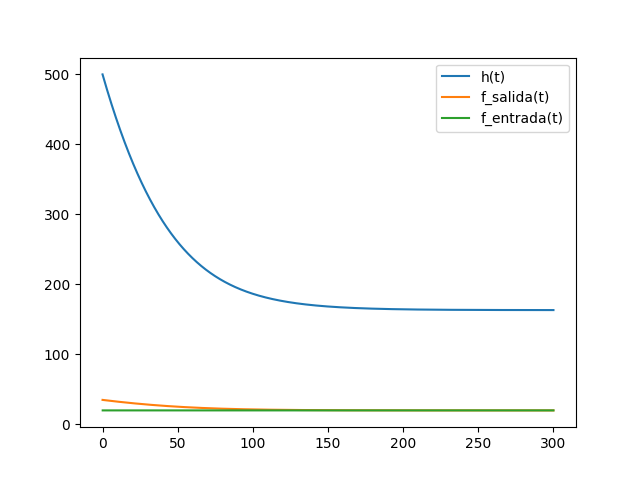
\includegraphics[width=\linewidth]{c20k05}
		\caption{$K = 0.5$}
		\label{gr:c20k0.5}
	\end{minipage}
	\begin{minipage}{0.32\textwidth}
		\centering
		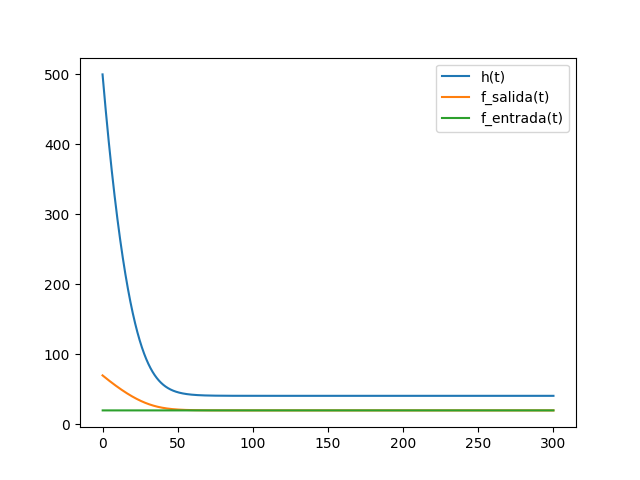
\includegraphics[width=\linewidth]{c20k1}
		\caption{$K = 1$}
		\label{gr:c20k1}
	\end{minipage}
	\begin{minipage}{0.32\textwidth}
		\centering
		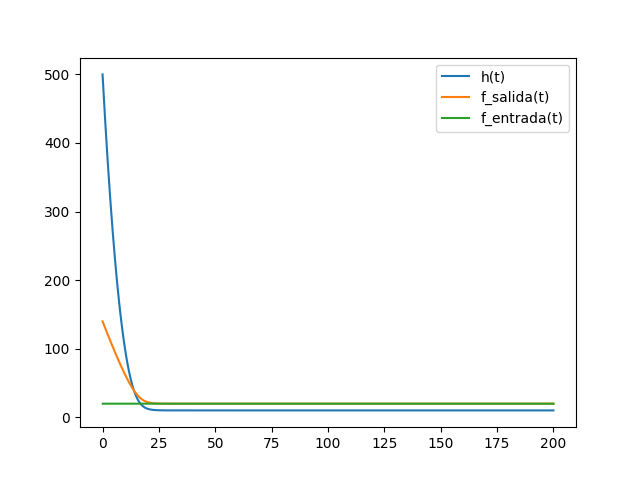
\includegraphics[width=\linewidth]{c20k2}
		\caption{$K = 2$}
		\label{gr:c20k2}
	\end{minipage}
\end{figure}

Cada figura difiere en que el caudal de salida está afectado por un factor multiplicativo diferente. En la Figura \ref{gr:c20k0.5}, el caudal de salida está multiplicado por $K=0.5$, y en la figura \ref{gr:c20k2}, por $K=2$.

Se observan los siguientes resultados para cada caudal de salida:
\begin{itemize}
  \item $k=0.5$: la altura se estabiliza despues de 265 unidades de tiempo en $h(t)=163$.
  \item $k=1$: la altura se estabiliza despues de 165 unidades de tiempo en $h(t)=41$.
  \item $k=2$: la altura se estabiliza despues de 125 unidades de tiempo en $h(t)=10$.
\end{itemize}

Algo similar ocurre cuando el caudal de salida es de 100 unidades por unidad de tiempo, como se observa en las figuras \ref{gr:c100k1}, \ref{gr:c100k0.5} y \ref{gr:c100k2}.

\begin{figure}[h]
	\begin{minipage}{0.32\textwidth}
		\centering
		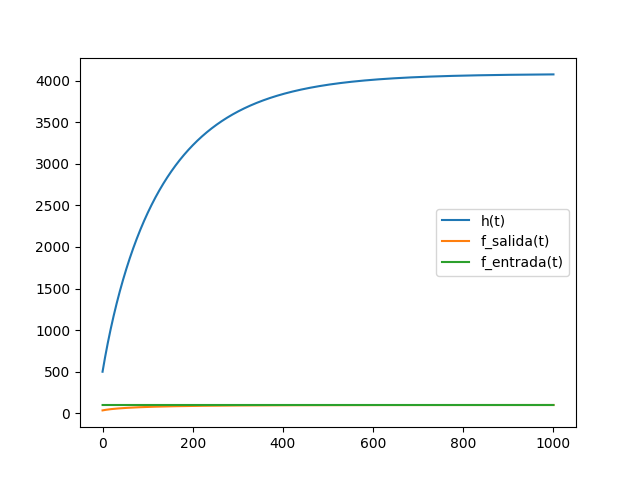
\includegraphics[width=\linewidth]{c100k05}
		\caption{$K = 0.5$}
		\label{gr:c100k0.5}
	\end{minipage}
	\begin{minipage}{0.32\textwidth}
		\centering
		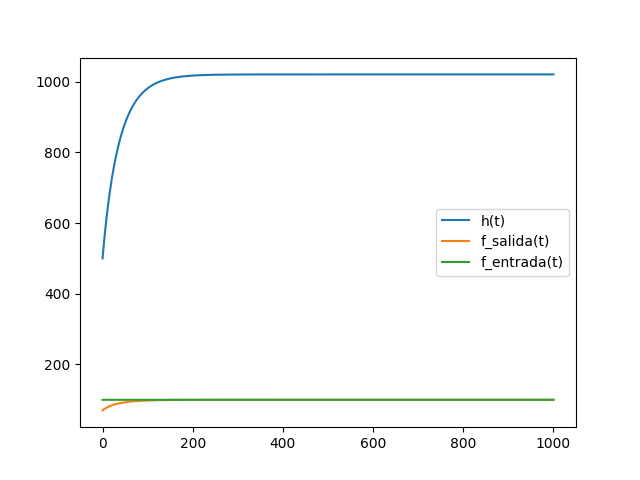
\includegraphics[width=\linewidth]{c100k1}
		\caption{$K = 1$}
		\label{gr:c100k1}
	\end{minipage}
	\begin{minipage}{0.32\textwidth}
		\centering
		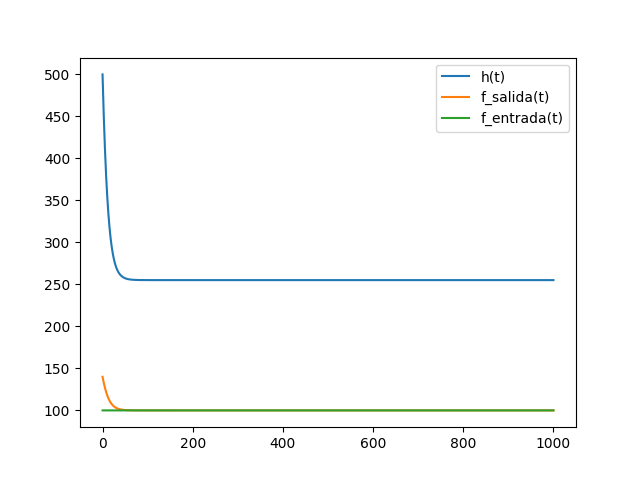
\includegraphics[width=\linewidth]{c100k2}
		\caption{$K = 2$}
		\label{gr:c100k2}
	\end{minipage}
\end{figure}

Los valores observados para cada caudal de salida son los siguientes:

\begin{itemize}
  \item $k=0.5$: la altura se estabiliza despues de 938 unidades de tiempo en $h(t)=4073$.
  \item $k=1$: la altura se estabiliza despues de 292.1 unidades de tiempo en $h(t)=1020$.
  \item $k=2$: la altura se estabiliza despues de 157.8 unidades de tiempo en $h(t)=255$.
\end{itemize}

Notar que para $k=1$ el sistema se estabiliza por debajo de la altura inicial, porque al comienzo del sistema la salida (f\_salida(t)) es mayor que la entrada (f\_entrada(t)).

Para ambas funciones constantes se observa que el punto de estabilidad se alcanza a medida que los caudales de entrada y salida se igualan.


\subsection*{Función de entrada variable}


A continuación se modela un tanque similar al del problema original, que presenta un sensor de la altura del líquido que no deja que el tanque se rebalse o se vacíe. Cuando el agua llega a la altura máxima de 800 unidades, desciende el caudal de entrada a 20. Posteriormente, cuando el sensor lee la altura en el umbral inferior de 200 unidades de altura, el flujo de entrada aumenta a 100.

La función de entrada es variable, dependiente del tiempo, de la altura del agua y de la velocidad de aumento de la altura (derivada), y está definida como

\[ \fosc(t) = \begin{cases}
		100 & h(t) < 800 \land h'(t) > 0 \\
		20  & h(t) \geq 800              \\
		100 & h(t) \leq 200              \\
		20  & h(t) > 200 \land h'(t) < 0
	\end{cases} \]

Esto quiere decir que el caudal de entrada es

\begin{itemize}
	\item 100 si la altura está por debajo de 800 y la altura está creciendo
	\item 20 si la altura alcanzó 800
	\item 100 si la altura alcanzó 200
	\item 20 si la altura está por encima de 200 y está bajando
\end{itemize}

El comportamiento de esta función de entrada se demuestra en la figura \ref{gr:osck1}.

\begin{figure}[ht] \centering
	\begin{minipage}{0.45\textwidth}
		\centering
		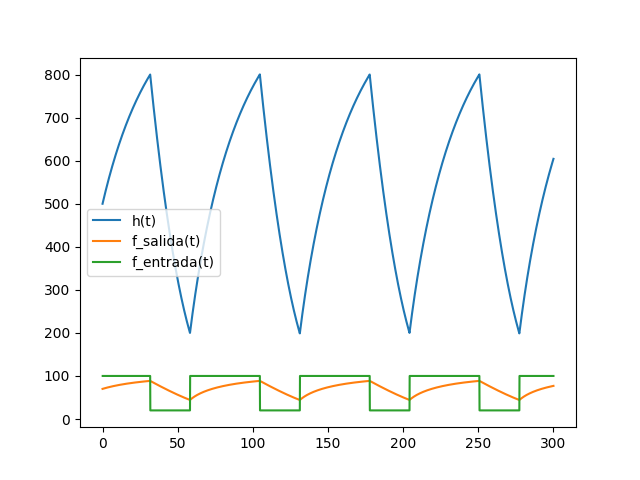
\includegraphics[width=\linewidth]{osck1}
		\caption{$k = 1$}
		\label{gr:osck1}
	\end{minipage}
	\begin{minipage}{0.45\textwidth}
		\centering
		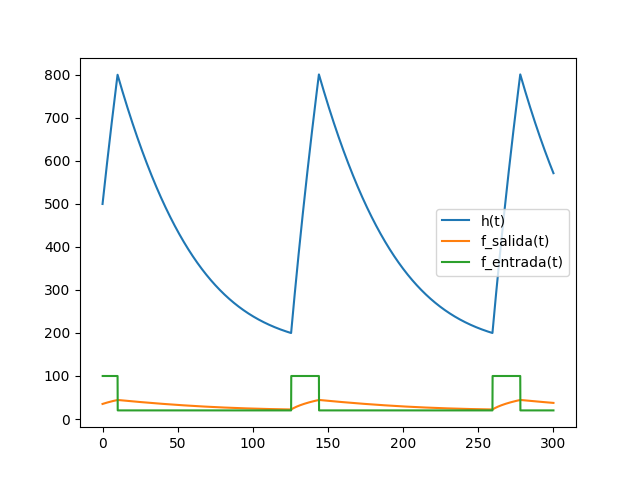
\includegraphics[width=\linewidth]{osck05}
		\caption{$k = 0.5$}
		\label{gr:osck05}
	\end{minipage}
\end{figure}

Se observa en la figura \ref{gr:osck05} que al disminuir el caudal de salida (afectado por $K=0.5$), el tanque tarda aproximadamente tres veces más en alcanzar el umbral inferior. Los puntos de estabilización están por fuera del rango (200,800), por lo que la altura nunca llega a estabilizarse, ya que el sensor causa que se cambie el caudal de entrada antes de ese punto.


\section*{Conclusión}


Debido a que el flujo de salida es proporcional a la altura del agua, se observa que el sistema se estabiliza cuando el caudal de entrada y el de salida son iguales. Además, si el caudal de entrada es mayor que el de salida, la altura del agua aumenta, y si el caudal de entrada es menor que el de salida, la altura del agua disminuye.

Cuando la función de entrada es constante, los flujos de entrada y de salida tienden a igualarse en un punto, y por lo tanto estabilizar el sistema. En el caso de la función de entrada oscilante, se evita que los caudales de entrada y de salida se igualen, lo que provoca que la altura del agua nunca se estabilice.

Por otro lado, al afectar el caudal de salida con un factor $K$, se observa que tanto la altura como el tiempo de estabilización son inversamente proporcionales a $K$. Es decir, al aumentar el factor del caudal de salida, disminuye el tiempo que tarda en llegar a una altura estable, la cual será menor también.

\end{document}
